% !TeX encoding = UTF-8
% Ban Chuong 4 doc lap, bien dich bang Tectonic / XeLaTeX / LuaLaTeX.
% Khi ghep vao bao cao: chi sao chep giua BEGIN CHAPTER BODY va END CHAPTER BODY.
% Giu cac anh trong picture/. Them bibitem coulter-pure-pursuit-1992 neu main.tex chua co.
% Khong thay doi main.tex. Du lieu: output/simulation_ch4; khong tao luot mo phong moi.
\documentclass[12pt,a4paper,oneside]{report}
\usepackage{fontspec}
\IfFontExistsTF{Times New Roman}{\setmainfont{Times New Roman}}{\setmainfont{TeX Gyre Termes}}
\setmonofont{Consolas}
\usepackage[left=3cm,right=2cm,top=2.5cm,bottom=2.5cm]{geometry}
\usepackage{amsmath,amssymb,graphicx,booktabs,array,enumitem,setspace,titlesec}
\usepackage[unicode,hidelinks]{hyperref}
\renewcommand{\chaptername}{Chương}
\renewcommand{\figurename}{Hình}
\renewcommand{\tablename}{Bảng}
\renewcommand{\bibname}{Tài liệu tham khảo}
\setcounter{secnumdepth}{2}
\setlength{\parindent}{1cm}
\setlength{\parskip}{4pt}
\setlength{\emergencystretch}{3em}
\setlist[itemize]{leftmargin=*,itemsep=3pt,topsep=4pt}
\setlist[enumerate]{leftmargin=*,itemsep=3pt,topsep=4pt}
\onehalfspacing
\graphicspath{{picture/}}
\titleformat{\chapter}[display]{\normalfont\bfseries\centering\Large}{\MakeUppercase{\chaptername}\ \thechapter}{8pt}{\Large}
\titlespacing*{\chapter}{0pt}{0pt}{18pt}
\titleformat{\section}{\normalfont\large\bfseries}{\thesection.}{0.5em}{}
\titleformat{\subsection}{\normalfont\normalsize\bfseries}{\thesubsection.}{0.5em}{}
\begin{document}
\setcounter{chapter}{3}

% ==================== BEGIN CHAPTER BODY ====================
\chapter{MÔ PHỎNG TÍCH HỢP, ĐÁNH GIÁ KẾT QUẢ VÀ ĐỀ XUẤT TRIỂN KHAI}
\label{chap:c4-doclap}

Chương này trình bày cấu hình robot mục tiêu, mô hình số và kết quả đánh giá chuỗi Dijkstra--Bézier bậc 2--Pure Pursuit--PI. Hai kịch bản được khảo sát là đi thẳng và tránh một vật cản tĩnh trên bản đồ biết trước. Phần quy hoạch cung cấp đường hình học và tham chiếu chuyển động; phần điều khiển sử dụng số đếm encoder để ước lượng tư thế và điều chỉnh vận tốc hai bánh.

\section{Cấu hình robot mục tiêu và mô hình mô phỏng}

\subsection{Cấu hình cơ khí, truyền động và encoder}

Robot mục tiêu là xe vi sai ba bánh, gồm hai bánh chủ động độc lập và một bánh tự lựa đỡ khung. Điểm tham chiếu \(P\) đặt tại trung điểm trục hai bánh chủ động; trục \(X_R\) hướng trước, \(Y_R\) hướng trái, chiều quay dương ngược chiều kim đồng hồ. Mô hình cơ sở sử dụng bán kính bánh danh định \(r_0=0{,}022\,\mathrm{m}\) và khoảng cách hai bánh \(L_0=0{,}135\,\mathrm{m}\).

\begin{center}
\begin{minipage}{\linewidth}
  \centering
  \refstepcounter{table}\label{tab:c4-hardware}
  \tablename~\thetable: Cấu hình robot mục tiêu và trạng thái sử dụng thông số\par\smallskip
  \small\singlespacing
  \renewcommand{\arraystretch}{1.22}
  \begin{tabular}{@{}>{\raggedright\arraybackslash}p{0.31\linewidth}>{\raggedright\arraybackslash}p{0.3\linewidth}>{\raggedright\arraybackslash}p{0.32\linewidth}@{}}
    \toprule
    \textbf{Hạng mục} & \textbf{Thông số} & \textbf{Căn cứ sử dụng}\\
    \midrule
    Vi điều khiển / driver & ESP32-C3-MINI / TB6612FNG & Kiến trúc phần cứng mục tiêu.\\
    Động cơ & GA12-N20, phiên bản 6 V; 300 RPM không tải & Thông tin được cung cấp; chưa dùng để nhận dạng mô hình truyền động.\\
    Bánh xe & Đường kính \(44\,\mathrm{mm}\); \(r_0=0{,}022\,\mathrm{m}\) & Giá trị danh định trong mô phỏng.\\
    Khoảng cách bánh & \(L_0=0{,}135\,\mathrm{m}\) & Giá trị danh định cho động học và Odometry.\\
    Encoder & Hall A/B; \(N_{\mathrm{eff}}=1400\) đếm/vòng đầu ra & Giả định giải mã x4 từ 7 chu kỳ/kênh và tỷ số truyền 50:1; cần kiểm tra trên xe.\\
    Nguồn động cơ & Thông tin cấu hình \(7{,}4\,\mathrm{V}\) & Chưa mô phỏng điện áp, dòng điện hoặc sụt áp nguồn.\\
    \bottomrule
  \end{tabular}
  
\end{minipage}
\end{center}


Hình~\ref{fig:c4-platform} minh họa bố trí nền tảng phần cứng. Hình này phục vụ mô tả cấu hình mục tiêu; bán kính thân bao dùng để kiểm tra va chạm trong mô phỏng được đặt riêng bằng \(0{,}11\,\mathrm{m}\). Khi triển khai trên xe, thân bao phải được xác định từ kích thước thực, có tính đến pin, mạch, bánh tự lựa và các phần nhô ra.

\begin{figure}[htbp]
  \centering
  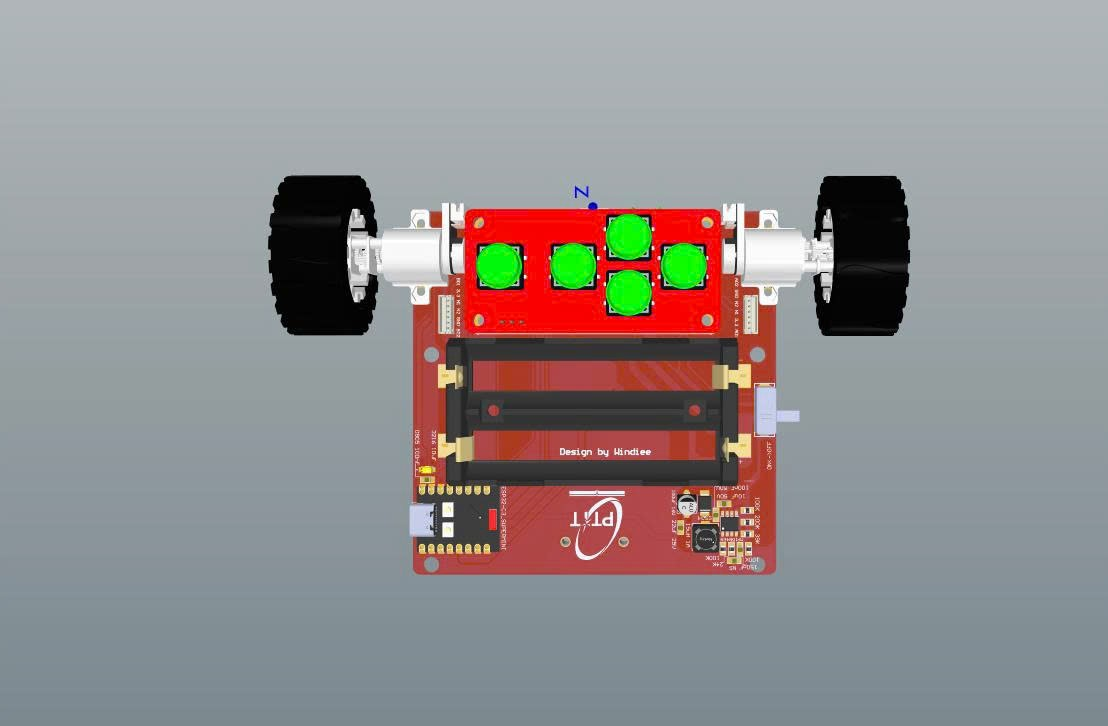
\includegraphics[width=0.67\linewidth]{Hinh_4_1_Mo_hinh_xe_3_banh.png}
  \caption{Minh họa nền tảng phần cứng mục tiêu cho xe vi sai; hình không được dùng thay cho phép đo kích thước và hiệu chuẩn}
  \label{fig:c4-platform}
\end{figure}


7 chu kỳ trên mỗi kênh encoder trước hộp số và tỷ số truyền 50:1, cách giải mã x1, x2, x4 lần lượt cho 350, 700, 1400 đếm trên một vòng đầu ra, nếu cách hiểu chu kỳ và tỷ số truyền là đúng. Mô phỏng chọn x4 với \(N_{\mathrm{eff}}=1400\). Bước quãng đường danh định tương ứng là
\begin{equation}
  \delta s=\frac{2\pi r_0}{N_{\mathrm{eff}}}
  \simeq 0{,}0987\,\mathrm{mm}/\text{đếm}.
  \label{eq:c4-encoder-resolution}
\end{equation}

\subsection{Phương án điện tử và phân chia tác vụ trên phần cứng}

Trong phương án triển khai, ESP32-C3-MINI được thiết kế để thu nhận encoder, cập nhật Odometry, chạy hai vòng điều khiển tốc độ và thực thi bộ quy hoạch cùng bước làm mượt. Máy tính có thể phục vụ nạp cấu hình, giám sát và ghi nhật ký. Việc phân chia này là kiến trúc mục tiêu; bộ số liệu được phân tích trong chương được tạo bởi chương trình Python trên máy tính, chưa cung cấp số đo thời gian xử lý hoặc RAM của bộ quy hoạch trên ESP32.

TB6612FNG cung cấp hai kênh cầu H cho hai động cơ. Phương án kết nối gồm hai tín hiệu PWM, bốn tín hiệu chiều và tín hiệu cho phép hoạt động; encoder hai bánh cung cấp bốn kênh A/B. PWM dự kiến được tạo bằng LEDC và số đếm được thu qua ngắt GPIO theo tài liệu ESP-IDF \cite{espressif-c3-peripherals}. Nguồn logic, mức tín hiệu encoder, chân phục vụ khởi động và chân nạp chương trình phải được đối chiếu với đúng phiên bản bo trước khi lắp.

\begin{figure}[htbp]
  \centering
  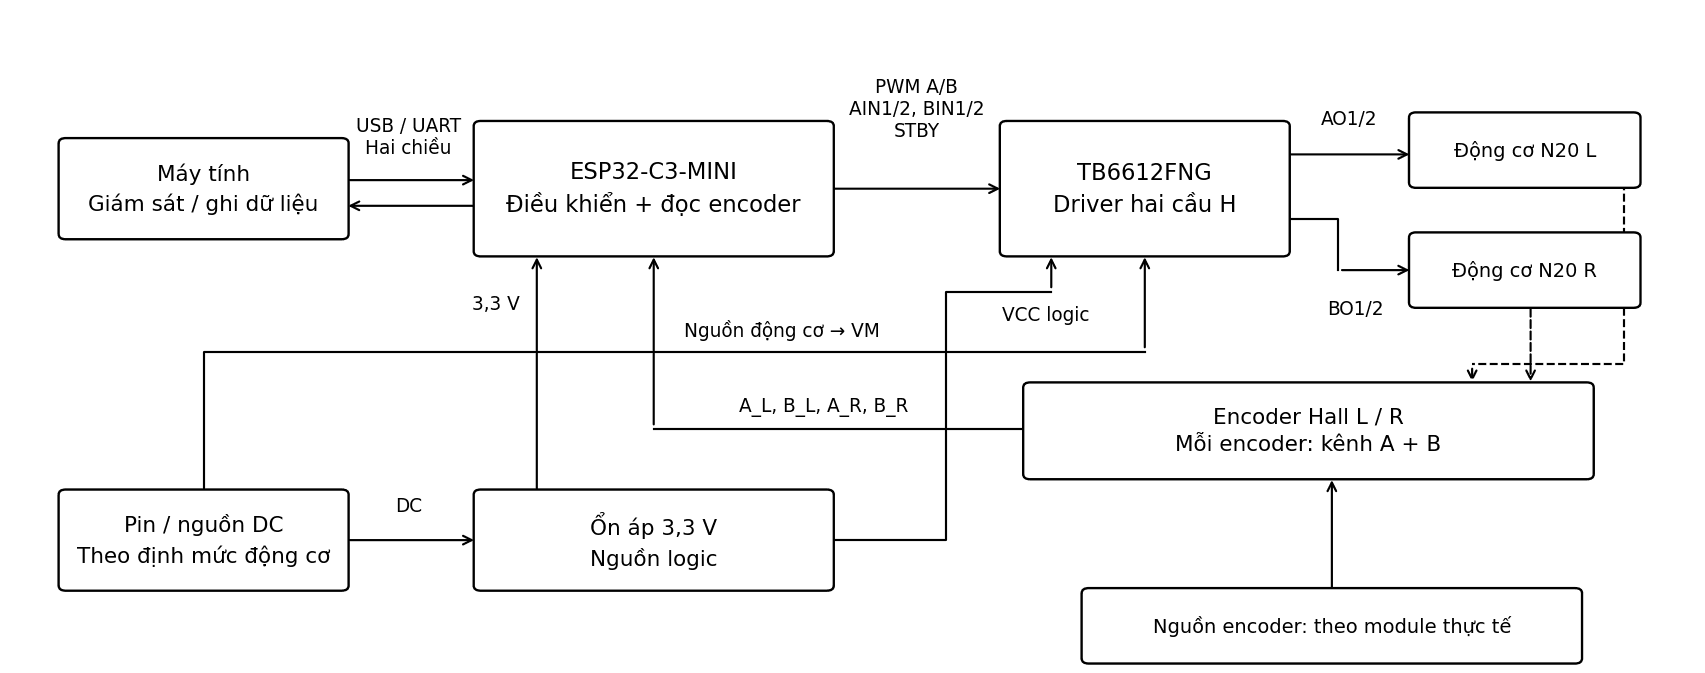
\includegraphics[width=\linewidth]{Hinh_4_2_Ket_noi_phan_cung.png}
  \caption{Sơ đồ kết nối điện tử dự kiến của hệ thống điều khiển và truyền động}
  \label{fig:c4-electronics}
\end{figure}


Phương án dùng nguồn logic \(3{,}3\,\mathrm{V}\); chế độ tiến, lùi, phanh và chờ của driver được lựa chọn theo bảng chức năng TB6612FNG \cite{toshiba-tb6612fng}. Thông tin nguồn động cơ \(7{,}4\,\mathrm{V}\) được giữ như điều kiện cấu hình phần cứng. Mô hình số chưa mô phỏng mạch điện, dòng điện, mô-men, nhiệt hoặc sụt áp, nên chưa dùng nguồn này để suy ra tải mang được, tốc độ dưới tải hay điện năng tiêu thụ.

\subsection{Mô hình truyền động và trạng thái đối chứng}

Mỗi bánh dùng mô hình đáp ứng vận tốc góc bậc nhất:
\begin{equation}
  \dot\Omega_i(t)=\frac{g_i u_i(t)-\Omega_i(t)}{\tau_i},
  \qquad \dot\phi_i(t)=\Omega_i(t),\quad i\in\{L,R\}.
  \label{eq:c4-motor-model}
\end{equation}
Trong đó \(u_i\) là duty có dấu, không thứ nguyên; \(\Omega_i\) là vận tốc góc trục bánh, \(\phi_i\) là góc quay tích lũy, \(g_i\) có đơn vị rad/s và \(\tau_i\) là hằng số thời gian. Hai giá trị danh định \(g_0=25\,\mathrm{rad/s}\), \(\tau_0=0{,}12\,\mathrm{s}\) được giả định để tạo mô hình thử. Chúng chưa được nhận dạng từ động cơ N20 ở điện áp 7,4 V.

Vận tốc hiệu dụng tác động lên chuyển động thân xe được biểu diễn bởi
\begin{equation}
  v_i^{*}=r_i^{*}\Omega_i\bigl(1-\lambda_i(t)\bigr),\qquad
  v^{*}=\frac{v_R^{*}+v_L^{*}}{2},\qquad
  \omega^{*}=\frac{v_R^{*}-v_L^{*}}{L^{*}}.
  \label{eq:c4-effective-velocity}
\end{equation}
Dấu \(*\) chỉ tham số hoặc trạng thái thật của mô hình số, phân biệt với tham số danh định dùng trong bộ điều khiển. Hệ số \(\lambda_i\) là cách biểu diễn đơn giản ảnh hưởng trượt và nhiễu vận tốc tương đương; chưa phải mô hình lực tiếp xúc giữa lốp và sàn. Tư thế đối chứng thỏa
\begin{equation}
  \dot x^{*}=v^{*}\cos\theta^{*},\qquad
  \dot y^{*}=v^{*}\sin\theta^{*},\qquad
  \dot\theta^{*}=\omega^{*}.
  \label{eq:c4-truth-kinematics}
\end{equation}
Trạng thái này chỉ được dùng để tính sai số và kiểm tra va chạm, không phản hồi vào Pure Pursuit hoặc PI. Khi thân bao chạm vùng cấm, bộ giám sát mô phỏng dừng lượt chạy. Cơ chế dừng mô phỏng này chưa chứng minh robot thật có khả năng tự phát hiện vật cản.

\begin{center}
\begin{minipage}{\linewidth}
  \centering
  \refstepcounter{table}\label{tab:c4-config}
  \tablename~\thetable: Thông số cố định của mô hình và bộ điều khiển trong 60 lượt chạy\par\smallskip
  \small\singlespacing
  \renewcommand{\arraystretch}{1.22}
  \begin{tabular}{@{}>{\raggedright\arraybackslash}p{0.48\linewidth}>{\raggedright\arraybackslash}p{0.46\linewidth}@{}}
    \toprule
    \textbf{Đại lượng} & \textbf{Giá trị đã sử dụng}\\
    \midrule
    Bán kính đĩa bao thân xe & \(r_b=0{,}11\,\mathrm{m}\), giả định hình học\\
    Hệ số / hằng số thời gian truyền động & \(g_0=25\,\mathrm{rad/s}\); \(\tau_0=0{,}12\,\mathrm{s}\)\\
    Chu kỳ PI / chu kỳ Pure Pursuit & \(0{,}01\,\mathrm{s}\) / \(0{,}05\,\mathrm{s}\)\\
    Bước tích phân mô hình chuyển động & \(0{,}0025\,\mathrm{s}\)\\
    Cửa sổ đo vận tốc từ số đếm & \(0{,}05\,\mathrm{s}\)\\
    Khoảng nhìn trước & \(L_{\mathrm{fw}}=0{,}20\,\mathrm{m}\), cố định\\
    Hệ số PI & \(K_P=2\,\mathrm{s/m}\); \(K_I=8\,\mathrm{m}^{-1}\); \(K_D=0\)\\
    Giới hạn duty chuẩn hóa & \(|u_i|\leq0{,}8\)\\
    Tốc độ dọc đường / gia tốc đặt & \(v_{\max}=0{,}25\,\mathrm{m/s}\); \(a=0{,}20\,\mathrm{m/s^2}\)\\
    Giới hạn tốc độ bánh / tốc độ quay thân & \(0{,}35\,\mathrm{m/s}\) / \(1{,}5\,\mathrm{rad/s}\)\\
    Ngưỡng chuyển pha theo Odometry & Vị trí \(0{,}015\,\mathrm{m}\); hướng \(0{,}025\,\mathrm{rad}\)\\
    Thời gian chờ ổn định cuối lượt & Ít nhất \(0{,}5\,\mathrm{s}\); vận tốc hai bánh nhỏ\\
    Số lượt / giới hạn thời gian & 30 lượt/kịch bản; \(35\,\mathrm{s}\)/lượt\\
    \bottomrule
  \end{tabular}
  \par\smallskip\begin{minipage}{0.97\linewidth}\footnotesize Các hệ số PI ứng với sai số vận tốc dài và duty không thứ nguyên trong mô hình số; chưa phải thông số đã hiệu chỉnh trên robot.\end{minipage}
\end{minipage}
\end{center}


Mỗi lượt lấy mẫu đều độc lập cho bán kính hai bánh và khoảng cách bánh trong phạm vi \(\pm1\%\), hệ số truyền động trong \(\pm5\%\), hằng số thời gian trong \(\pm15\%\). Hệ số trượt nền mỗi bánh thuộc \([0;0{,}02]\), cộng dao động biên độ \(0{,}002\), tần số \(0{,}7\,\mathrm{Hz}\) và pha ngẫu nhiên. Hệ số tức thời có thể khác miền của giá trị nền do thành phần dao động; nó được dùng như nhiễu vận tốc tương đương trong mô hình đơn giản.

\clearpage
\section{Thuật toán và cấu hình điều khiển trong mô phỏng}

\subsection{Chuỗi quy hoạch, làm mượt và tạo tham chiếu}

Bản đồ được biết trước, vật cản đứng yên. Dijkstra tìm đường trên lưới tám hướng với bước \(0{,}05\,\mathrm{m}\), cấm đi chéo xuyên góc và kiểm tra các đoạn nối. Robot được bao bởi đĩa bán kính \(0{,}11\,\mathrm{m}\); khoảng cách tâm xe tới vật cản khi quy hoạch tối thiểu là \(0{,}26\,\mathrm{m}\), gồm thân bao và khoảng dự phòng \(0{,}15\,\mathrm{m}\). Biên bản đồ cũng được xét trong miền hoạt động hợp lệ. Tính tối ưu của Dijkstra chỉ áp dụng cho đồ thị và trọng số đã xây dựng \cite{lavalle-planning-2006}.

Đường được rút gọn bằng nối tắt có kiểm tra, sau đó bo góc bằng Bézier bậc 2 theo phương pháp ở Chương 2. Khoảng lùi tối đa là \(0{,}15\,\mathrm{m}\), đồng thời không quá 40\% chiều dài mỗi đoạn kề. Nếu đoạn bo chưa đạt khoảng hở yêu cầu thì giảm khoảng lùi một nửa, tối đa 14 lần thử. Các đoạn cong được kiểm tra tại 301 giá trị tham số và toàn bộ đường sau xử lý được kiểm tra lại với khoảng cách tâm tới vật cản ít nhất \(0{,}21\,\mathrm{m}\). Đây là kiểm tra rời rạc của cài đặt hiện tại, chưa phải chứng nhận không va chạm liên tục cho mọi hình học.

Bézier bậc 2 được dùng để liên tục hướng tiếp tuyến tại góc bo trên đường lý tưởng; phương án chưa bảo đảm \(G^2/C^2\) ở chỗ nối với đoạn thẳng. Đường sau xử lý được lưu theo chiều dài cung với bước khoảng \(0{,}005\,\mathrm{m}\). Hướng tham chiếu là hướng tiếp tuyến; hướng đích là tiếp tuyến cuối của đường. Từ quy luật vận tốc hình thang danh định, vị trí tham chiếu theo thời gian có dạng
\begin{equation}
  \mathbf p_d(t)=\mathbf p\bigl(s_d(t)\bigr),\qquad
  s_d(t)=\int_0^t v_d(\tau)\,d\tau.
  \label{eq:c4-time-reference}
\end{equation}
Sau thời gian chuyển động danh định, tham chiếu được giữ tại đích để tính sai số cho phần thời gian còn lại.

\begin{figure}[htbp]
  \centering
  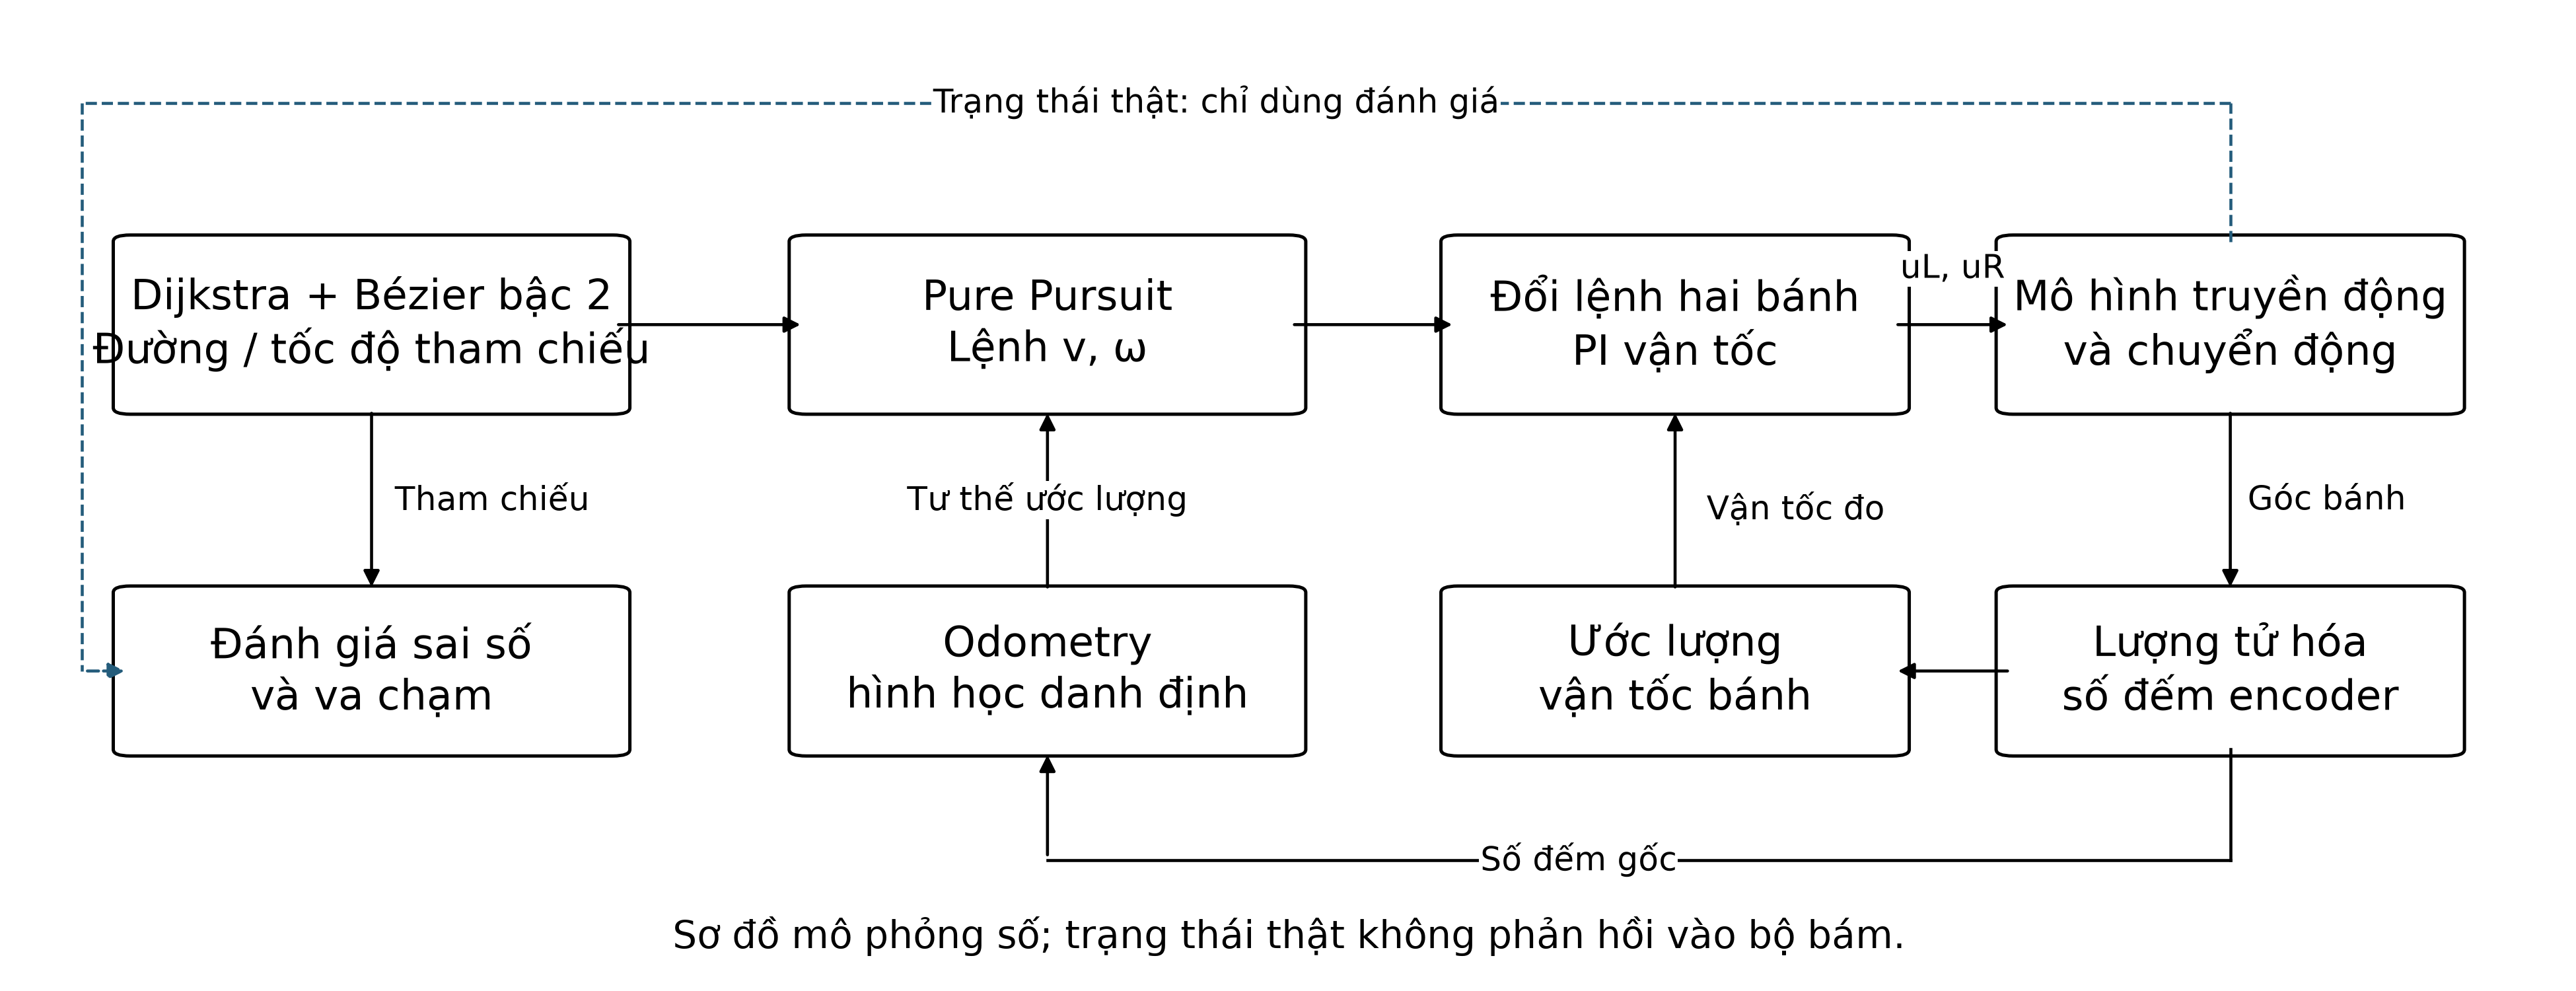
\includegraphics[width=\linewidth]{Chuong4_Kien_truc_mo_phong.png}
  \caption{Luồng thông tin trong mô phỏng tích hợp; trạng thái thật đi vào khối đánh giá, không vào bộ điều khiển bám}
  \label{fig:c4-simulation-architecture}
\end{figure}


\subsection{Odometry và ước lượng vận tốc từ encoder}

Mô hình encoder lượng tử hóa góc quay thành số đếm:
\begin{equation}
  n_i=\operatorname{round}\!\left(\frac{N_{\mathrm{eff}}\phi_i}{2\pi}\right),\qquad
  \Delta\widehat s_i=\frac{2\pi r_0\Delta n_i}{N_{\mathrm{eff}}}.
  \label{eq:c4-counts-to-distance}
\end{equation}
Odometry dùng \(r_0,L_0\) danh định, trong khi chuyển động đối chứng dùng \(r_i^{*},L^{*}\) và hệ số trượt. Vì encoder quan sát góc quay trục bánh, thông tin này chưa đủ để nhận biết riêng quãng dịch chuyển bị ảnh hưởng bởi trượt. Số đếm mô phỏng chưa xét mất ngắt hoặc nhiễu điện của encoder thật.

Độ lệch vị trí ngang ban đầu thuộc \(\pm0{,}02\,\mathrm{m}\), độ lệch hướng ban đầu thuộc \(\pm0{,}05\,\mathrm{rad}\) so với tuyến tham chiếu. Odometry được khởi tạo đúng bằng tư thế thật tại đầu lượt, vì vậy mô phỏng chưa khảo sát bất định định vị ban đầu. Các sai lệch hình học và trượt phát sinh trong quá trình chuyển động không được bộ điều khiển biết trước. Hai kịch bản dùng cùng seed cho từng cặp lượt để giữ điều kiện sai lệch tương ứng.

Đặt
\begin{equation}
  \Delta\widehat s=\frac{\Delta\widehat s_R+\Delta\widehat s_L}{2},\qquad
  \Delta\widehat\theta=\frac{\Delta\widehat s_R-\Delta\widehat s_L}{L_0}.
  \label{eq:c4-odom-increments}
\end{equation}
Giả thiết chuyển động xoắn không đổi trong chu kỳ, công thức cung tròn cập nhật tư thế là
\begin{equation}
  \begin{aligned}
    \widehat x_{k+1}&=\widehat x_k+\Delta\widehat s\,
       \operatorname{sinc}(\Delta\widehat\theta/2)
       \cos(\widehat\theta_k+\Delta\widehat\theta/2),\\
    \widehat y_{k+1}&=\widehat y_k+\Delta\widehat s\,
       \operatorname{sinc}(\Delta\widehat\theta/2)
       \sin(\widehat\theta_k+\Delta\widehat\theta/2),\\
    \widehat\theta_{k+1}&=\widehat\theta_k+\Delta\widehat\theta,
  \end{aligned}
  \label{eq:c4-odom-update}
\end{equation}
trong đó \(\operatorname{sinc}(z)=\sin z/z\), \(\operatorname{sinc}(0)=1\). Vận tốc phản hồi cho PI được tính từ chênh lệch số đếm trên cửa sổ tối đa 50 ms. Vị trí vẫn tích lũy từ số đếm gốc, tránh làm mất quãng đường do lọc hoặc kéo dài cửa sổ vận tốc.

\subsection{Pure Pursuit, giới hạn lệnh và điều kiện dừng}

Pure Pursuit chọn điểm phía trước trên đường, dựa trên tư thế Odometry và thứ tự tiến triển, với khoảng nhìn trước cố định \(L_{\mathrm{fw}}=0{,}20\,\mathrm{m}\). Hình học của thuật toán được trình bày trong báo cáo gốc của Coulter \cite{coulter-pure-pursuit-1992}. Với điểm nhìn trước có tọa độ \((x_g^R,y_g^R)\) trong hệ thân xe, cài đặt sử dụng
\begin{equation}
  \kappa_{\mathrm{pp}}=
  \frac{2y_g^R}{\max\{(x_g^R)^2+(y_g^R)^2,\varepsilon^2\}},
  \qquad \varepsilon=0{,}001\,\mathrm{m}.
  \label{eq:c4-pure-pursuit}
\end{equation}
Điểm nhìn trước được chọn theo nhánh tiến triển. Công thức dùng khoảng cách thực tới điểm đó; chặn mẫu số chỉ phục vụ xử lý số, chưa chứng minh ổn định.

\begin{samepage}
Trong pha bám đường, gọi \(\widehat s\) là tiến triển ước lượng và \(D\) là chiều dài tuyến. Lệnh trước giới hạn chung được tính bởi
\begin{equation}
  \widetilde v_c=\min\!\left\{v_{\max},at,
                 \sqrt{2a\max(D-\widehat s,0)}\right\},
  \qquad \widetilde\omega_c=\widetilde v_c\kappa_{\mathrm{pp}}.
  \label{eq:c4-speed-law}
\end{equation}
\end{samepage}
Sau đó giảm đồng thời hai lệnh theo hệ số
\begin{equation}
  \begin{aligned}
  \gamma=\max\!\left\{1,\frac{|\widetilde\omega_c|}{\omega_{\max}},
       \frac{|\widetilde v_c-L_0\widetilde\omega_c/2|}{v_{w,\max}},
       \frac{|\widetilde v_c+L_0\widetilde\omega_c/2|}{v_{w,\max}}\right\},\\
  v_c=\widetilde v_c/\gamma,\qquad
  \omega_c=\widetilde\omega_c/\gamma.
  \end{aligned}
  \label{eq:c4-command-scaling}
\end{equation}
Giá trị \(a=0{,}20\,\mathrm{m/s^2}\) xác định quy luật tăng tốc và khoảng dừng dự kiến. Do lệnh còn thay đổi theo tiến triển, độ cong và các pha chuyển trạng thái, giá trị này chưa tự chứng minh mọi thành phần gia tốc bánh hoặc thân xe đều được chặn ở cùng mức.

Khi khoảng cách Odometry tới đích không quá \(0{,}015\,\mathrm{m}\), bộ điều khiển chuyển sang căn hướng với lệnh quay được giới hạn trong \(\pm0{,}5\,\mathrm{rad/s}\). Khi sai số hướng ước lượng nhỏ hơn \(0{,}025\,\mathrm{rad}\), hệ chuyển sang chờ dừng; lượt kết thúc sau ít nhất 0,5 s và khi vận tốc hai bánh, quy đổi theo bán kính danh định, nhỏ hơn \(0{,}01\,\mathrm{m/s}\). Điều kiện này được đánh giá trên ước lượng nội bộ, khác điều kiện đạt theo trạng thái đối chứng ở mục 4.3.

Pure Pursuit trong cấu hình này chủ yếu bám hình học. Lệnh tốc độ điều chỉnh theo tiến triển thực có thể khác lịch hình thang danh định trong \eqref{eq:c4-time-reference}. Vì vậy, sai số hình học tới đường và sai số vị trí theo cùng thời điểm được đánh giá riêng; chưa khẳng định bộ bám bảo đảm đồng bộ thời gian của toàn quỹ đạo.

\subsection{PI vận tốc hai bánh và duty PWM}

Động học nghịch cho hai lệnh vận tốc dài:
\begin{equation}
  v_R^{\mathrm{ref}}=v_c+\frac{L_0\omega_c}{2},\qquad
  v_L^{\mathrm{ref}}=v_c-\frac{L_0\omega_c}{2}.
  \label{eq:c4-wheel-references}
\end{equation}
Với \(e_{i,k}=v_{i,k}^{\mathrm{ref}}-\widehat v_{i,k}\), mỗi vòng PI cập nhật ở 100 Hz theo
\begin{equation}
  I_{i,k}=I_{i,k-1}+e_{i,k}\Delta t,\qquad
  u_{i,k}^{*}=K_Pe_{i,k}+K_II_{i,k},\qquad
  u_{i,k}=\operatorname{clip}(u_{i,k}^{*},-0{,}8,0{,}8).
  \label{eq:c4-pi}
\end{equation}
Dấu của duty quy định chiều quay, trị tuyệt đối quy định mức điều khiển chuẩn hóa. Mô phỏng dùng PI với \(K_D=0\), chưa có bù thuận hoặc chống bão hòa tích phân. Chỉ chặn đầu ra chưa ngăn tích phân tiếp tục tăng khi bão hòa; tuy nhiên cần dựa trên dữ liệu để xác định hiện tượng đó có xuất hiện trong lượt khảo sát hay không.

Khi chuyển lên xe, cần kiểm tra dấu phản hồi, PWM và chế độ dừng/phanh theo driver. Các hệ số PI mô phỏng cần được hiệu chỉnh bằng dữ liệu đáp ứng thực.

\clearpage
\section{Kết quả mô phỏng tích hợp và phân tích sai số}

\subsection{Kịch bản, dữ liệu và tiêu chí đánh giá}

Miền mô phỏng có kích thước \(4{,}0\times2{,}4\,\mathrm{m}\), điểm đầu \(S=(0{,}3;1{,}2)\,\mathrm{m}\), đích \(G=(3{,}3;1{,}2)\,\mathrm{m}\). Kịch bản thứ nhất dùng đường thẳng dài 3 m. Kịch bản thứ hai có vật cản chữ nhật \([1{,}4;2{,}0]\times[0{,}85;1{,}55]\,\mathrm{m}\), chắn đường nối trực tiếp. Đường tránh vật cản sau xử lý dài khoảng \(3{,}41198\,\mathrm{m}\), với khoảng hở thân bao tới vật cản tối thiểu khoảng \(0{,}16574\,\mathrm{m}\).

\begin{figure}[htbp]
  \centering
  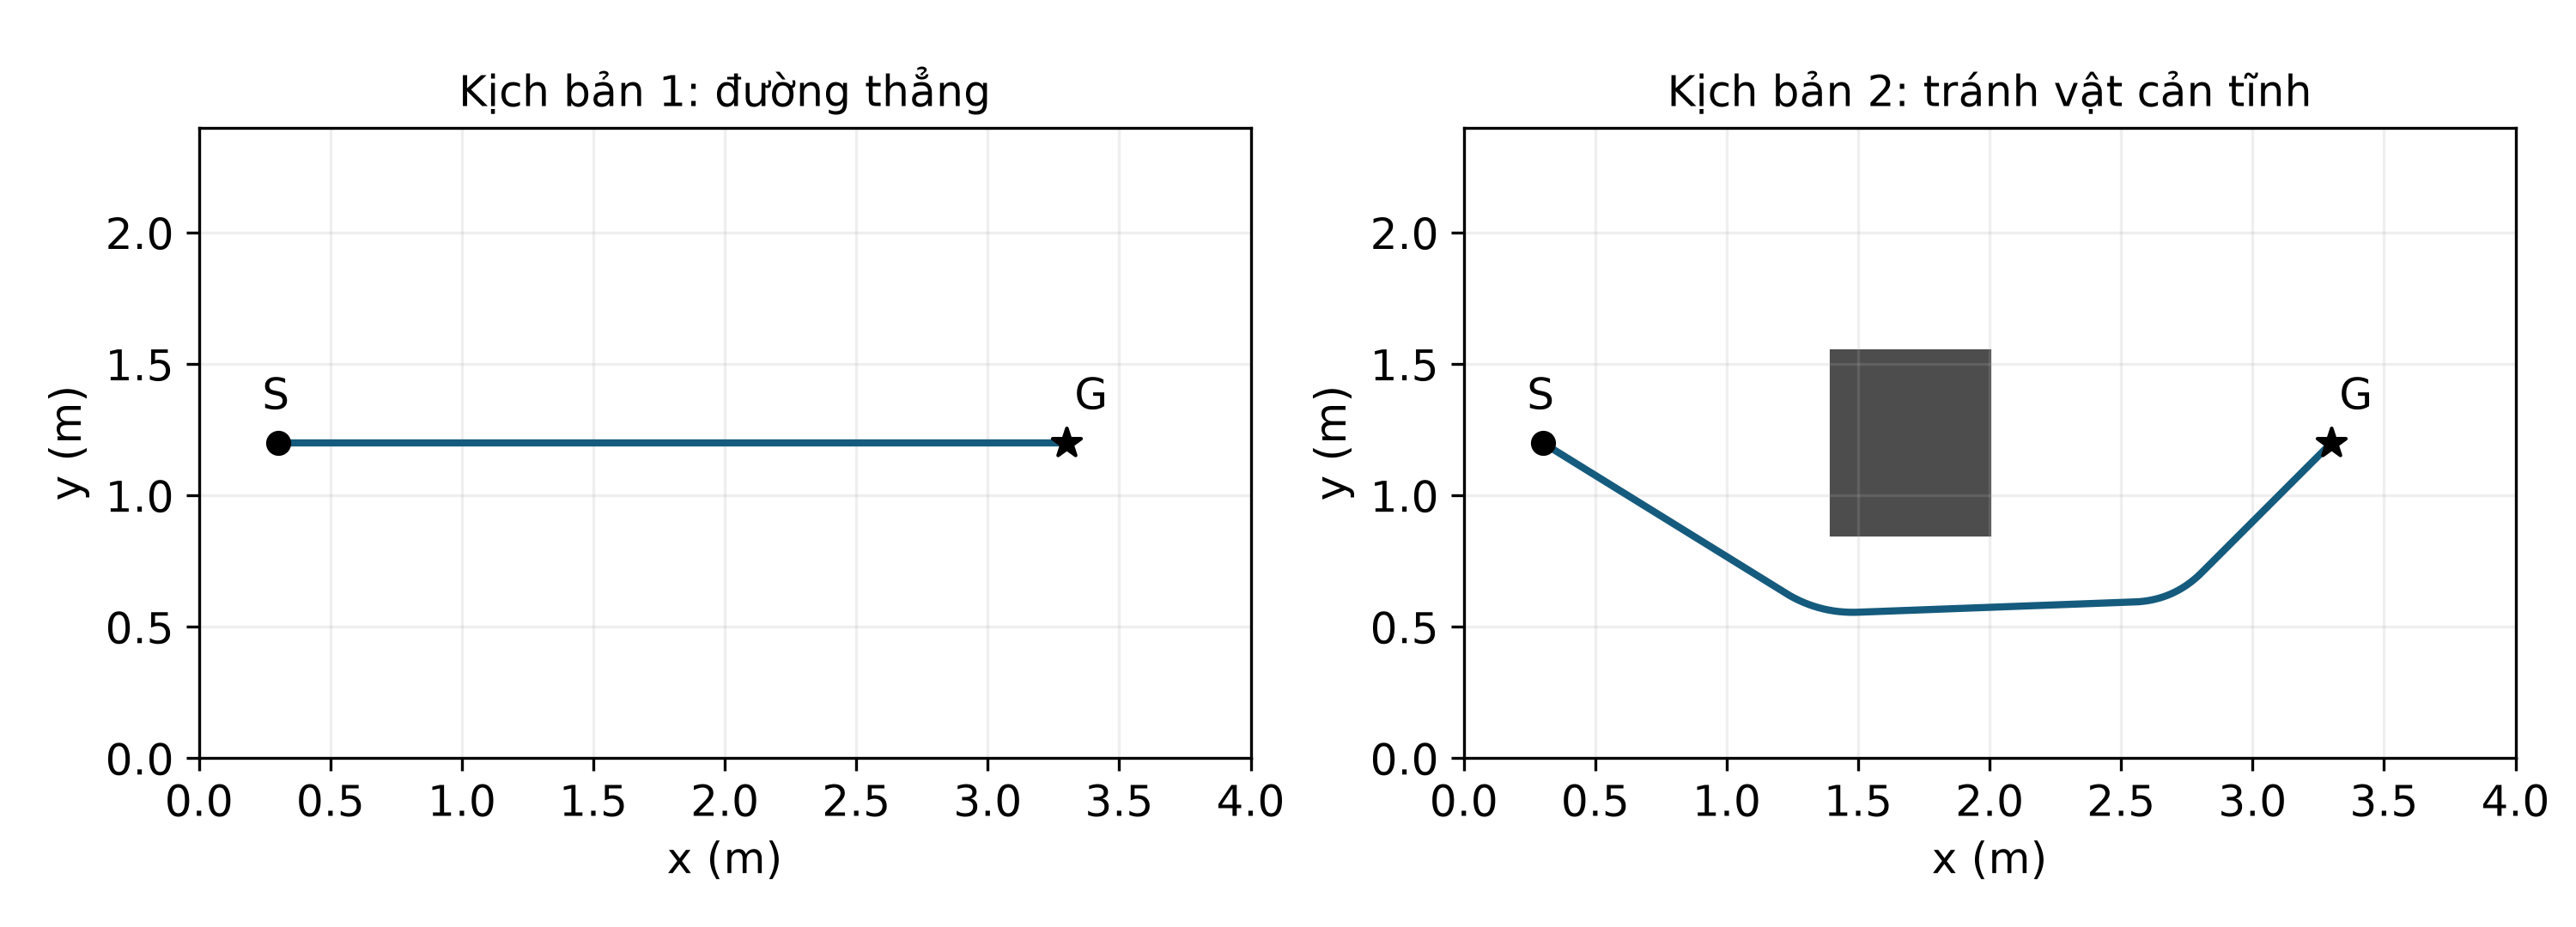
\includegraphics[width=\linewidth]{Chuong4_Kich_ban_mo_phong.png}
  \caption{Hai đường tham chiếu được sử dụng trong mô phỏng; hình được vẽ từ tệp đường tham chiếu đã lưu}
  \label{fig:c4-scenarios}
\end{figure}


Mỗi kịch bản gồm 30 lượt, seed từ 20261031 đến 20261060, sử dụng cùng cấu trúc điều khiển. Nhật ký ở 100 Hz gồm thời gian, tư thế thật của mô hình, Odometry, số đếm, vận tốc đặt và đo hai bánh, duty trước/sau giới hạn, sai số ngang và khoảng hở. Mỗi lượt được giữ nguyên trạng thái kết thúc: bộ điều khiển hoàn tất, va chạm hoặc hết thời gian. Không loại lượt không đạt khỏi tổng số thử.

Một lượt đạt khi bộ điều khiển hoàn tất trong 35 s, khoảng cách vị trí thật đến đích không quá \(0{,}05\,\mathrm{m}\), sai số hướng cuối không quá \(0{,}10\,\mathrm{rad}\), sai số ngang lớn nhất không quá \(0{,}15\,\mathrm{m}\) và không va chạm. Sai số hướng được bọc về \([-\pi,\pi]\) và so với tiếp tuyến cuối đường. Các ngưỡng này là điều kiện đánh giá của phép thử, chưa được xác nhận như dung sai ứng dụng công nghiệp.

Mô phỏng kiểm tra khoảng hở tại từng bước tích phân 0,0025 s và dừng nếu khoảng hở không dương. Ngưỡng sai số ngang 0,15 m dùng để chấm đạt, chưa phải một cơ chế chủ động dừng xe trong bộ điều khiển hiện tại. Việc bộ giám sát dừng lượt sau va chạm không được diễn giải thành khả năng né vật cản trực tuyến.

Với \(\mathbf p_k^{*}\) là vị trí thật và \(\mathbf p_{d,k}\) là tham chiếu tại cùng thời điểm, RMSE vị trí của một lượt là
\begin{equation}
  \mathrm{RMSE}_p=\sqrt{\frac{1}{N}\sum_{k=1}^{N}
                     \|\mathbf p_k^{*}-\mathbf p_{d,k}\|^2}.
  \label{eq:c4-rmse}
\end{equation}
Sai số ngang lấy theo đoạn tham chiếu gần nhất có xét đúng nhánh tiến triển. Sai số cuối được tính tại thời điểm lượt dừng, kể cả khi va chạm. Lượt dừng sớm chỉ dùng các mẫu đã có, không bổ sung mẫu bằng không. Những quy ước này giúp giữ nguyên thông tin thất bại khi tổng hợp.

Mã mô phỏng nằm trong thư mục \path{code/simulation_ch4}; bộ dữ liệu gốc tại \path{output/simulation_ch4}. Hồ sơ gồm cấu hình, tham số từng lượt, chỉ tiêu tổng hợp và CSV nhật ký để truy xuất kết quả. Các phân tích bổ sung dưới đây được tính từ nhật ký đã lưu, không phát sinh lượt mô phỏng mới.

\subsection{Kết quả tổng hợp và mức đáp ứng dung sai}

\begin{center}
\begin{minipage}{\linewidth}
  \centering
  \refstepcounter{table}\label{tab:c4-results}
  \tablename~\thetable: Kết quả mô phỏng tích hợp trên toàn bộ lượt chạy\par\smallskip
  \small\singlespacing
  \renewcommand{\arraystretch}{1.22}
  \begin{tabular}{@{}>{\raggedright\arraybackslash}p{0.44\linewidth}>{\raggedright\arraybackslash}p{0.24\linewidth}>{\raggedright\arraybackslash}p{0.25\linewidth}@{}}
    \toprule
    \textbf{Chỉ tiêu} & \textbf{Đường thẳng} & \textbf{Có vật cản}\\
    \midrule
    Số lượt đạt / tổng số lượt & 5/30 & 5/30\\
    Tỷ lệ đạt & \(16{,}7\%\) & \(16{,}7\%\)\\
    RMSE vị trí theo thời gian (m) & \(0{,}167\pm0{,}118\) & \(0{,}167\pm0{,}121\)\\
    Sai số ngang lớn nhất (m) & \(0{,}897\) & \(0{,}677\)\\
    Sai số hướng tuyệt đối trung bình (rad) & \(0{,}101\pm0{,}089\) & \(0{,}116\pm0{,}087\)\\
    Sai số vị trí khi kết thúc (m) & \(0{,}293\pm0{,}267\) & \(0{,}404\pm0{,}450\)\\
    Thời gian hoàn thành của lượt đạt (s) & \(13{,}762\pm0{,}022\) & \(15{,}416\pm0{,}035\)\\
    Số lượt va chạm & 0 & 3\\
    Khoảng hở thân xe nhỏ nhất (m) & Không áp dụng & \(-0{,}00025\)\\
    Thời gian PWM bão hòa (\%) & \(0{,}000\pm0{,}000\) & \(0{,}000\pm0{,}000\)\\
    \bottomrule
  \end{tabular}
  \par\smallskip\begin{minipage}{0.97\linewidth}\footnotesize Các giá trị có dấu \(\pm\) là trung bình và độ lệch chuẩn mẫu của 30 lượt, trừ thời gian hoàn thành chỉ dùng 5 lượt đạt. Sai số ngang lớn nhất và khoảng hở nhỏ nhất là cực trị trên tất cả lượt. Sai số cuối của lượt va chạm được tính tại thời điểm dừng.\end{minipage}
\end{minipage}
\end{center}


Cả hai kịch bản đều có 5 lượt đạt trong 30 lượt, tương ứng 16,7\%. Trên đường thẳng, toàn bộ 30 lượt kết thúc theo điều kiện dừng nội bộ, nhưng 25 lượt không đạt ít nhất một tiêu chí đối chứng. Trong kịch bản có vật cản, 27 lượt kết thúc theo điều kiện của bộ điều khiển, 3 lượt dừng do va chạm; trong 27 lượt hoàn tất, chỉ 5 lượt đạt đầy đủ các điều kiện.

RMSE vị trí trung bình xấp xỉ 0,167 m ở hai kịch bản. Sai số vị trí cuối trung bình là 0,293 m trên đường thẳng và 0,404 m khi có vật cản. Hai giá trị này vượt dung sai đích 0,05 m và có độ phân tán lớn. Vì vậy, cấu hình khảo sát chưa đáp ứng ổn định yêu cầu điểm dừng đã đặt, mặc dù các bộ điều khiển phần lớn báo hoàn tất nhiệm vụ.

Thời gian 13,762 s và 15,416 s chỉ mô tả nhóm 5 lượt đạt ở mỗi kịch bản, bao gồm căn hướng và chờ ổn định. Không dùng thời gian này để kết luận tốc độ hoàn thành của toàn bộ 30 lượt hoặc đánh đổi hiệu quả với một bộ điều khiển khác chưa được khảo sát.

Khoảng hở âm khoảng 0,25 mm biểu thị độ xuyên số rất nhỏ tại bước phát hiện va chạm; 3 lượt va chạm vẫn được tính là không đạt. Đối với kịch bản có vật cản, khoảng hở được kiểm tra tới cả vật cản và biên bản đồ. PWM không chạm giới hạn trong các lượt khảo sát, nhưng điều này chưa chứng minh động cơ thật không quá dòng hoặc hệ thống luôn đủ công suất, vì mô hình chưa có đại lượng điện và tải cơ tương ứng.

Hình~\ref{fig:c4-existing-results} giữ các đường đã chạy và diễn biến sai số từ dữ liệu gốc. Lượt đại diện là lượt 10 của kịch bản đường thẳng và lượt 25 của kịch bản có vật cản, được chọn theo vị trí trung vị trên của RMSE trong 30 lượt. Cách chọn này phản ánh một mức sai số điển hình theo chỉ tiêu đã xác định, không chỉ chọn lượt thành công.

\begin{figure}[htbp]
  \centering
  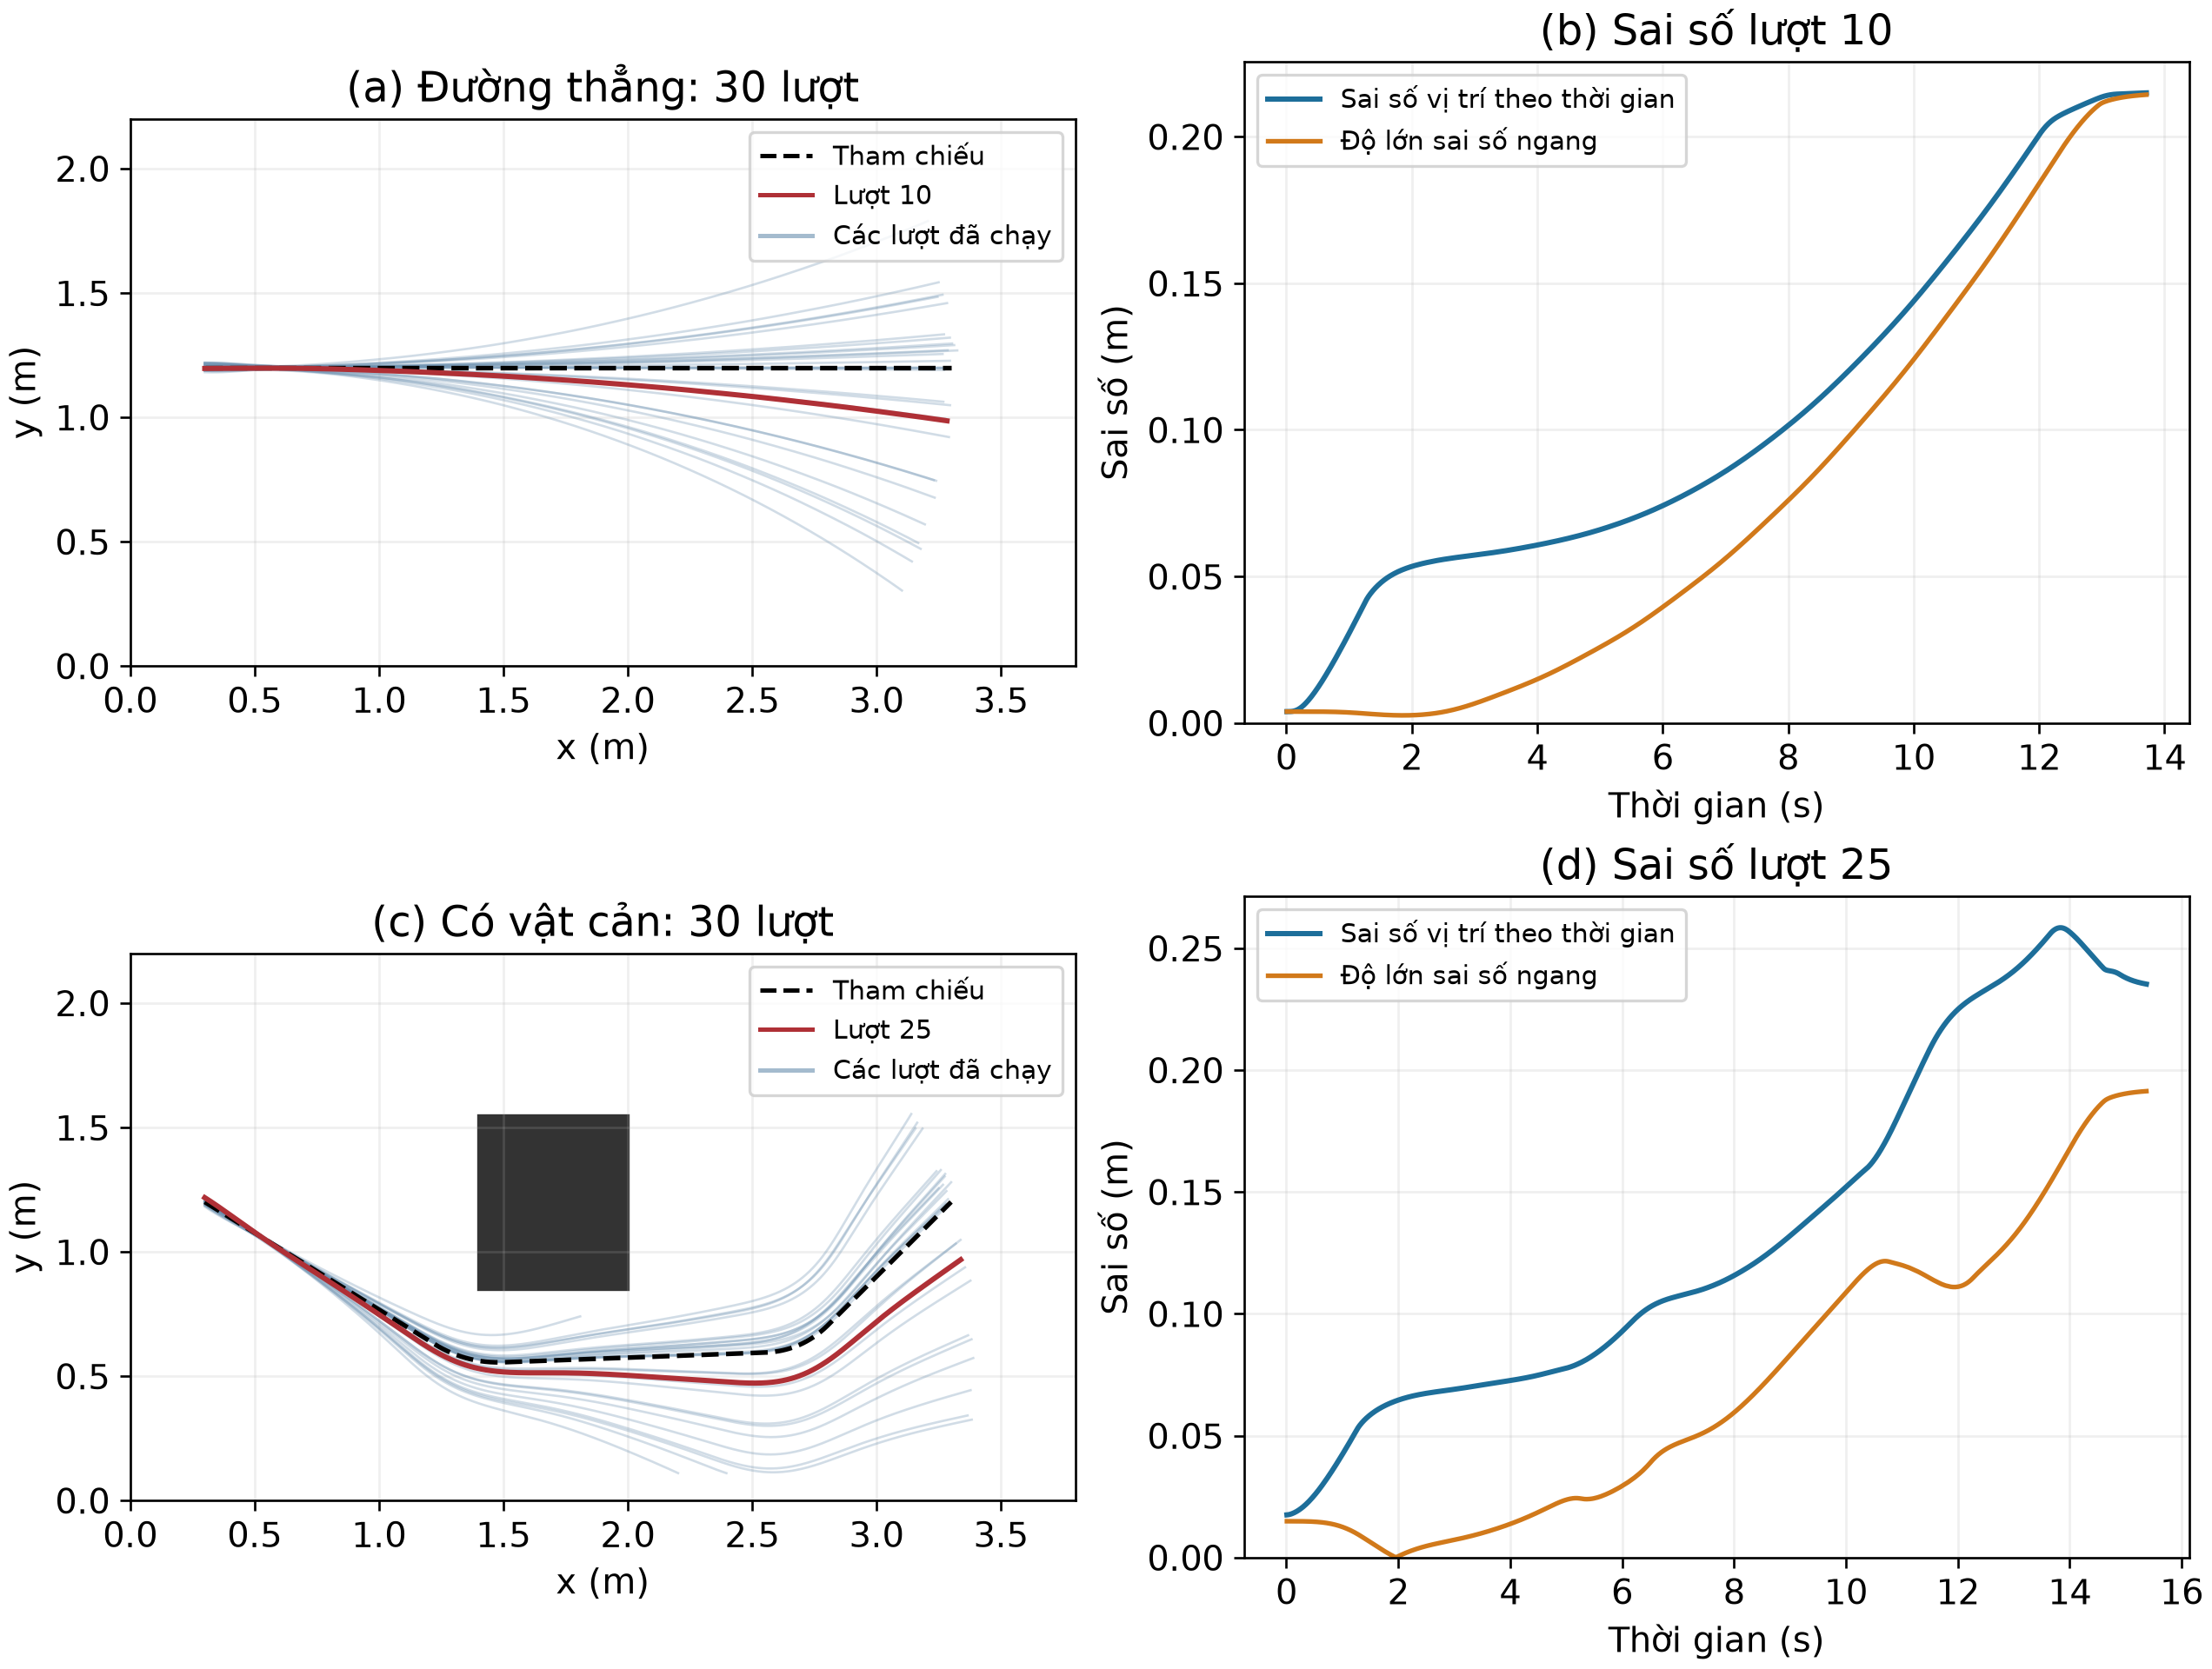
\includegraphics[width=\linewidth]{Hinh_4_5_Ket_qua_mo_phong.png}
  \caption{Đường chuyển động của 30 lượt và sai số của lượt đại diện trong từng kịch bản, giữ nguyên dữ liệu mô phỏng gốc}
  \label{fig:c4-existing-results}
\end{figure}


\subsection{Phân loại các điều kiện không đạt}

\begin{center}
\begin{minipage}{\linewidth}
  \centering
  \refstepcounter{table}\label{tab:c4-failures}
  \tablename~\thetable: Số lượt vi phạm từng điều kiện đánh giá\par\smallskip
  \small\singlespacing
  \renewcommand{\arraystretch}{1.22}
  \begin{tabular}{@{}>{\raggedright\arraybackslash}p{0.48\linewidth}>{\raggedright\arraybackslash}p{0.22\linewidth}>{\raggedright\arraybackslash}p{0.23\linewidth}@{}}
    \toprule
    \textbf{Điều kiện bị vi phạm} & \textbf{Đường thẳng} & \textbf{Có vật cản}\\
    \midrule
    Sai số vị trí cuối \(>0{,}05\,\mathrm{m}\) & 25/30 & 25/30\\
    Sai số hướng cuối \(>0{,}10\,\mathrm{rad}\) & 16/30 & 18/30\\
    Sai số ngang lớn nhất \(>0{,}15\,\mathrm{m}\) & 17/30 & 16/30\\
    Va chạm & 0/30 & 3/30\\
    Hết thời gian & 0/30 & 0/30\\
    \bottomrule
  \end{tabular}
  \par\smallskip\begin{minipage}{0.97\linewidth}\footnotesize Một lượt có thể vi phạm đồng thời nhiều điều kiện; không cộng các hàng để xác định tổng số lượt không đạt. Các giá trị được đếm lại từ chỉ tiêu từng lượt, không phải kết quả của một phép mô phỏng mới.\end{minipage}
\end{minipage}
\end{center}


Ở mỗi kịch bản, cả 25 lượt không đạt đều vượt dung sai vị trí cuối. Ngoài ra, một phần trong các lượt này còn vượt ngưỡng hướng hoặc sai số ngang. Vì vậy, sai lệch điểm dừng là nội dung cần phân tích trước, đồng thời phải xét các trường hợp lệch khỏi đường dẫn tới va chạm. Bảng phân loại xác định điều kiện bị vi phạm, chưa tách được đóng góp nhân quả của sai lệch bán kính, khoảng cách bánh, trượt hoặc đáp ứng truyền động.

Việc Dijkstra tạo ra một đường tham chiếu có khoảng hở dương chưa đủ để bảo đảm robot thực hiện đường đó an toàn khi tư thế ước lượng bị lệch. Kết quả 16,7\% đánh giá toàn chuỗi trong cấu hình có sai lệch; chưa đủ để quy nguyên nhân cho riêng bộ tìm đường hoặc cho riêng bộ PI.

\subsection{Đối chiếu sai số định vị và sai số theo tham chiếu}

Để phân biệt chất lượng ước lượng với chất lượng bám theo thời gian, đặt
\begin{equation}
  \begin{aligned}
  e_{\mathrm{loc}}(t)&=\|\mathbf p^{*}(t)-\widehat{\mathbf p}(t)\|,\\
  e_{\mathrm{odo,ref}}(t)&=\|\widehat{\mathbf p}(t)-\mathbf p_d(t)\|,\\
  e_{\mathrm{true,ref}}(t)&=\|\mathbf p^{*}(t)-\mathbf p_d(t)\|.
  \end{aligned}
  \label{eq:c4-error-decomposition}
\end{equation}
Ba đại lượng là độ lớn của các vectơ sai lệch, nên không cộng trực tiếp các độ lớn thành một đẳng thức. Chúng thỏa bất đẳng thức tam giác \(e_{\mathrm{true,ref}}\leq e_{\mathrm{loc}}+e_{\mathrm{odo,ref}}\). Hai chỉ tiêu so với \(\mathbf p_d(t)\) còn chứa ảnh hưởng robot tiến nhanh hoặc chậm hơn lịch danh định, khác sai số ngang tới đường.

\begin{center}
\begin{minipage}{\linewidth}
  \centering
  \refstepcounter{table}\label{tab:c4-localization}
  \tablename~\thetable: Đối chiếu vị trí ở nhóm kết thúc theo điều kiện của bộ điều khiển\par\smallskip
  \small\singlespacing
  \renewcommand{\arraystretch}{1.22}
  \begin{tabular}{@{}>{\raggedright\arraybackslash}p{0.43\linewidth}>{\raggedright\arraybackslash}p{0.25\linewidth}>{\raggedright\arraybackslash}p{0.25\linewidth}@{}}
    \toprule
    \textbf{Đại lượng} & \textbf{Đường thẳng} & \textbf{Có vật cản}\\
    \midrule
    Số lượt được sử dụng & 30 & 27\\
    Khoảng cách Odometry đến đích (m) & \(0{,}0146\pm0{,}0007\) & \(0{,}0146\pm0{,}0015\)\\
    Khoảng cách vị trí thật mô hình đến đích (m) & \(0{,}2929\pm0{,}2668\) & \(0{,}2818\pm0{,}2633\)\\
    Chênh lệch vị trí thật và Odometry (m) & \(0{,}2969\pm0{,}2651\) & \(0{,}2852\pm0{,}2654\)\\
    \bottomrule
  \end{tabular}
  \par\smallskip\begin{minipage}{0.97\linewidth}\footnotesize Trung bình \(\pm\) độ lệch chuẩn mẫu, tính từ mẫu cuối của CSV. Nhóm có vật cản loại 3 lượt dừng do va chạm theo đúng phạm vi thống kê của bảng này; Bảng~\ref{tab:c4-results} vẫn giữ đủ 30 lượt.\end{minipage}
\end{minipage}
\end{center}


Trong nhóm hoàn tất theo bộ điều khiển, khoảng cách Odometry tới đích trung bình chỉ khoảng 0,0146 m ở hai kịch bản, phù hợp với ngưỡng chuyển pha 0,015 m. Tuy nhiên, khoảng cách vị trí đối chứng tới đích vẫn khoảng 0,2929 m trên đường thẳng và 0,2818 m ở 27 lượt hoàn tất của kịch bản có vật cản. Sai lệch thật--Odometry cuối lượt tương ứng khoảng 0,2969 m và 0,2852 m. Các số liệu này cho thấy điều kiện dừng dựa trên tư thế ước lượng có thể được thỏa trong khi vị trí đối chứng còn lệch đáng kể.

\begin{figure}[htbp]
  \centering
  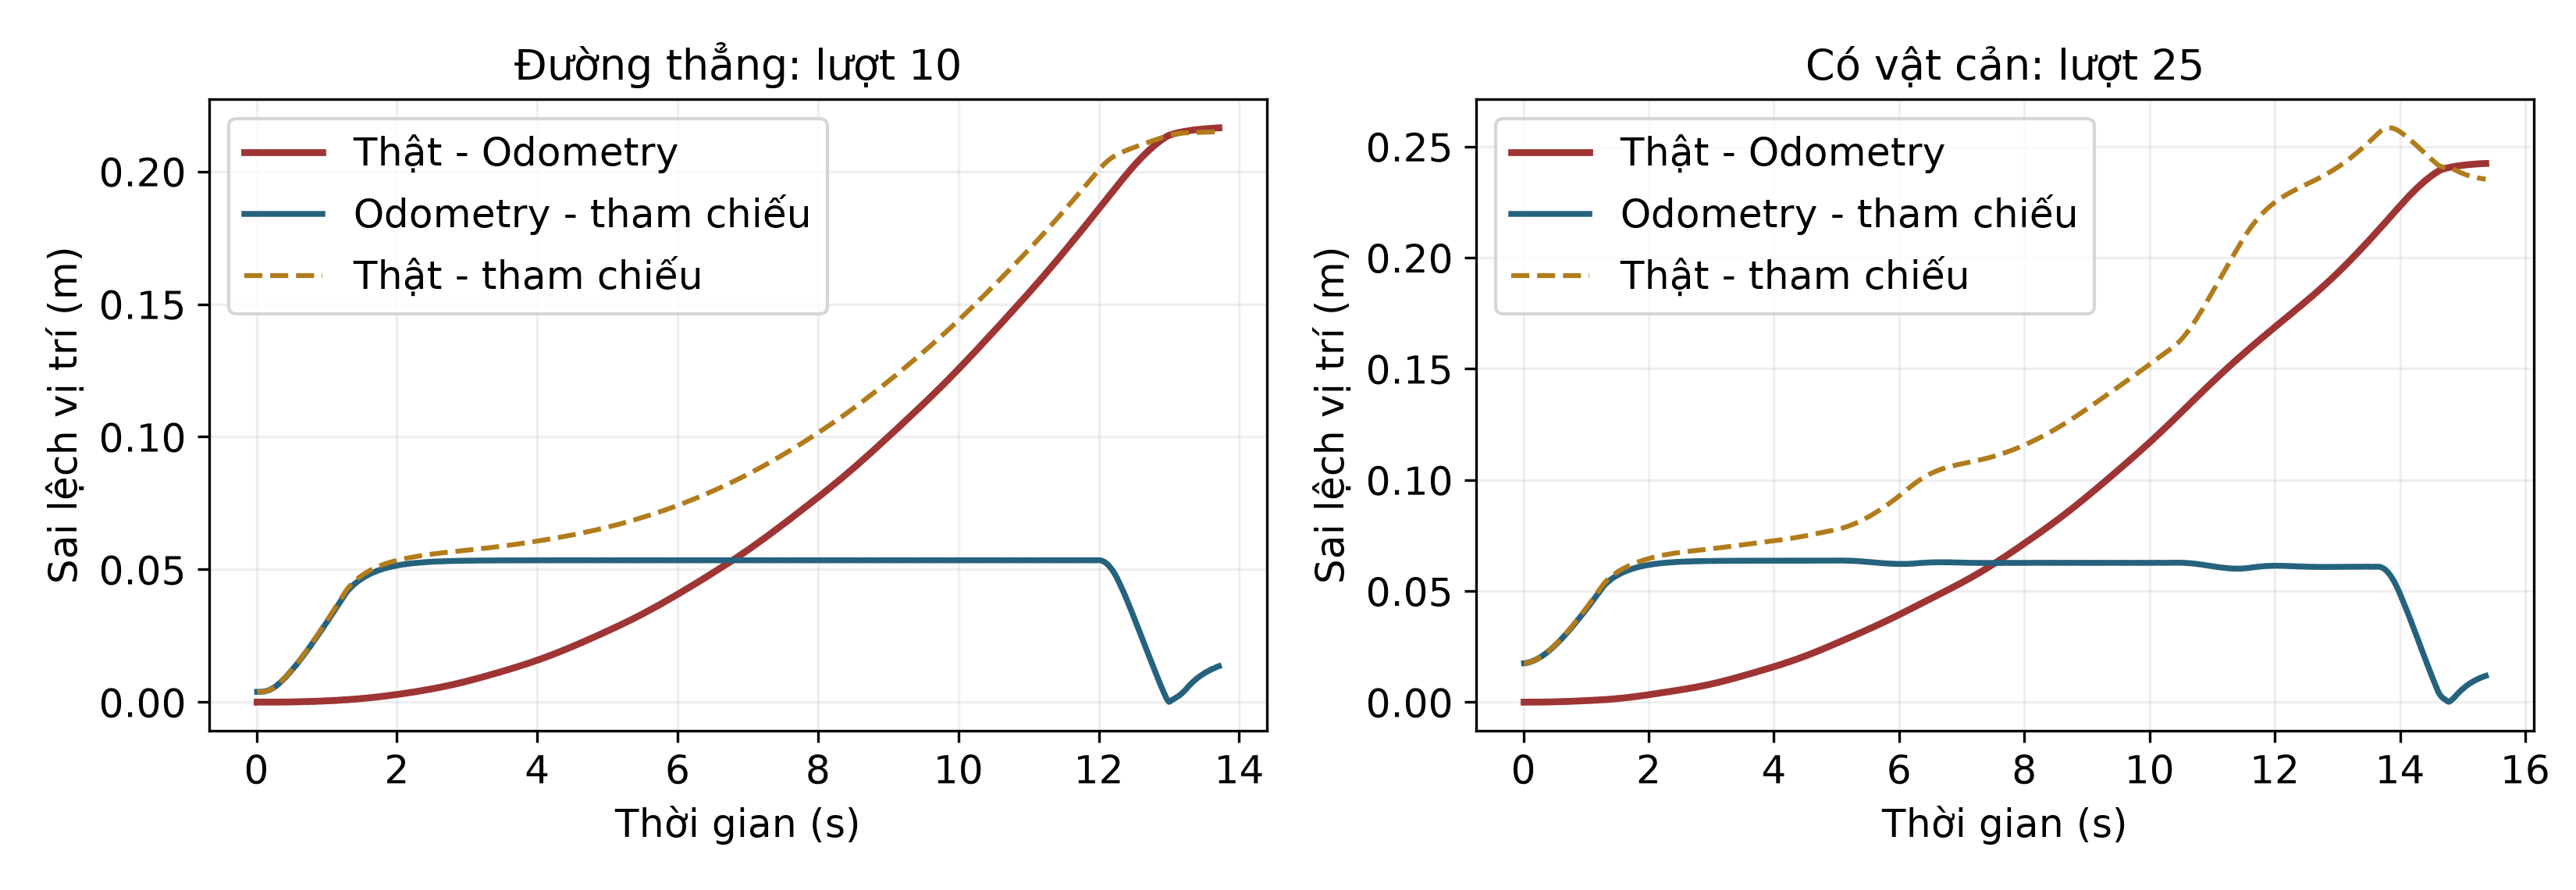
\includegraphics[width=\linewidth]{Chuong4_Phan_tich_Odometry.png}
  \caption{Đối chiếu ba sai lệch vị trí trên cùng hai lượt đại diện; đồ thị được tính lại từ nhật ký đã lưu và lịch tham chiếu danh định}
  \label{fig:c4-odometry-analysis}
\end{figure}


Trên hai lượt đại diện, sai lệch thật--Odometry tăng dần, trong khi sai lệch Odometry--tham chiếu có xu hướng giảm khi tới đích. Quan sát này hỗ trợ ưu tiên kiểm tra chất lượng ước lượng tư thế và hiệu chuẩn hình học. Tuy vậy, các nguồn sai lệch đang được thay đổi đồng thời, nên chưa thể lượng hóa riêng mức ảnh hưởng của từng nguồn hoặc kết luận hiệu chuẩn hình học đủ để loại bỏ sai số do trượt.

Các kiểm tra số đã lưu gồm: trường hợp đi thẳng lý tưởng cho sai lệch ngang cực đại bằng 0; kiểm tra khoảng hở đường mượt; so sánh giảm đôi bước tích phân ở seed đầu của mỗi kịch bản; và tính lại chỉ tiêu từ CSV. Sai khác RMSE khi giảm bước tích phân từ 0,0025 xuống 0,00125 s nhỏ hơn \(10^{-6}\,\mathrm{m}\) trong hai lượt kiểm tra; sai khác lớn nhất khi tính lại các chỉ tiêu từ CSV nhỏ hơn \(10^{-9}\). Đây là kiểm tra tính nhất quán tính toán, chưa phải xác nhận mô hình vật lý hoặc thay thế bộ thí nghiệm đối chứng đầy đủ.

\clearpage
\section{Giới hạn và phương án kiểm chứng tiếp theo}

\subsection{Giới hạn của kết quả hiện có}

Hai kịch bản sử dụng bản đồ tĩnh biết trước và mô hình thân bao tròn. Chưa mô phỏng cảm biến phát hiện vật cản, định vị theo bản đồ, SLAM, quy hoạch lại hoặc vật cản động. Bánh tự lựa, độ rơ hộp số, biến dạng lốp, tải thay đổi, điện áp pin và nhiễu điện cũng chưa được mô hình hóa đầy đủ. Hệ số trượt là giả định gây sai lệch vận tốc, chưa được suy ra từ phép đo lực hoặc nhận dạng tiếp xúc.

Tư thế đầu được biết đúng; các tham số thật và số đếm mô phỏng được tạo bởi mô hình đã đặt. Vì vậy, kết quả chỉ mô tả độ nhạy của cấu hình trong miền tham số khảo sát, chưa dự báo trực tiếp tỷ lệ đạt của xe thật. Số liệu hiện có chưa đủ để kết luận chuyển động êm hơn, tiết kiệm năng lượng, đáp ứng thời gian thực trên ESP32 hoặc sẵn sàng vận chuyển hàng hóa.

\subsection{Thiết kế đối chứng và đánh giá sau hiệu chỉnh}

\begin{center}
\begin{minipage}{\linewidth}
  \centering
  \refstepcounter{table}\label{tab:c4-ablation}
  \tablename~\thetable: Thiết kế phép đối chứng cần thực hiện tiếp\par\smallskip
  \small\singlespacing
  \renewcommand{\arraystretch}{1.22}
  \begin{tabular}{@{}>{\raggedright\arraybackslash}p{0.13\linewidth}>{\raggedright\arraybackslash}p{0.38\linewidth}>{\raggedright\arraybackslash}p{0.42\linewidth}@{}}
    \toprule
    \textbf{Cấu hình} & \textbf{Yếu tố thay đổi} & \textbf{Câu hỏi kiểm chứng}\\
    \midrule
    A0 & Hình học danh định, không trượt; các điều kiện khác cố định. & Chuỗi điều khiển có đạt trong điều kiện lý tưởng hay không?\\
    A1 & Chỉ thay đổi hình học; tắt trượt và các biến thiên truyền động. & Sai lệch bán kính bánh và khoảng cách bánh gây ảnh hưởng bao nhiêu?\\
    A2 & Chỉ thay đổi hệ số trượt; giữ hình học và truyền động danh định. & Sai lệch do trượt biểu hiện thế nào khi encoder không quan sát được?\\
    A3 & Kết hợp sai lệch theo cấu hình hiện tại. & Mốc so sánh với kết quả 60 lượt đã có.\\
    A4 & Giữ mô hình thật của A3, cập nhật tham số ước lượng theo một quy trình hiệu chuẩn. & Hiệu chuẩn cải thiện sai số, tỷ lệ đạt và va chạm đến mức nào?\\
    \bottomrule
  \end{tabular}
  \par\smallskip\begin{minipage}{0.97\linewidth}\footnotesize Đây là kế hoạch khảo sát bổ sung. Chưa có bộ kết quả đầy đủ A0--A4 để kết luận mức cải thiện.\end{minipage}
\end{minipage}
\end{center}


Các cấu hình cần dùng chung bản đồ, điều kiện đạt, giới hạn chuyển động và cách tính chỉ tiêu. Với từng nguồn nhiễu đang khảo sát, dùng các seed và điều kiện khởi tạo được ghép cặp phù hợp; những yếu tố còn lại giữ cố định. Ngoài tỷ lệ đạt, cần báo cáo RMSE, sai số ngang, sai số cuối, sai lệch Odometry và va chạm trên đầy đủ lượt thử.

Ở cấu hình sau hiệu chuẩn, cần giữ nguyên tham số thật của mô hình có sai lệch và cập nhật đúng các tham số mà bộ ước lượng sử dụng. Đưa cả mô hình thật về danh định chỉ tạo ra điều kiện lý tưởng, chưa chứng minh phương pháp hiệu chuẩn khắc phục được sai lệch. Nếu tham số được chỉnh trên một tập lượt chạy, cần có tập kiểm tra riêng trước khi kết luận hiệu quả. Không đặt trước một tỷ lệ cải thiện khi chưa thực hiện phép đo.

\subsection{Lộ trình kiểm chứng trên robot ba bánh}

\begin{enumerate}[label=\arabic*.]
  \item \textbf{Xác nhận phần cứng và phép đo:} Chốt phiên bản bo, sơ đồ GPIO, nguồn logic/động cơ và chế độ dừng của driver. Kiểm tra dấu encoder, số đếm mỗi vòng và mức tín hiệu thực; đo bán kính lăn dưới tải và khoảng cách bánh hiệu dụng.
  \item \textbf{Hiệu chỉnh truyền động:} Đo đáp ứng thay đổi tốc độ của từng bánh, xác định miền duty và vùng chết. Đánh giá thời gian xác lập, sai số xác lập và bão hòa trước khi chọn PI; không chuyển nguyên hệ số của mô hình số sang xe rồi coi là đã hiệu chỉnh.
  \item \textbf{Kiểm tra Odometry độc lập:} Thực hiện các lượt đi thẳng, quay và hành trình khép kín có phép đo ngoài. Hiệu chỉnh tham số, sau đó đánh giá lại trên hành trình khác để kiểm tra khả năng áp dụng.
  \item \textbf{Đo tài nguyên trên ESP32:} Đối chiếu đường đi và trạng thái không có đường với máy tính, sau đó đo thời gian quy hoạch, RAM, thời gian xử lý encoder và độ ổn định chu kỳ điều khiển khi đồng thời ghi dữ liệu. Xác nhận cơ chế xử lý lệnh quá hạn và dừng bằng thử nghiệm tương ứng.
  \item \textbf{Thử nghiệm tích hợp:} Chạy đường thẳng trước, tiếp đến tuyến tránh vật cản tĩnh ở tốc độ thấp. Dùng camera đã hiệu chuẩn hoặc hệ đo ngoài để đánh giá vị trí; ghi tất cả lượt không đạt, đo khoảng hở và xác nhận khả năng dừng trước khi tăng tốc hoặc tăng tải.
\end{enumerate}

\subsection{Hướng ứng dụng và mở rộng}

Nền tảng ESP32-C3-MINI, TB6612 và N20 có thể phục vụ nghiên cứu điều hướng trong nhà ở quy mô nhỏ, chẳng hạn đi giữa các trạm thực hành hoặc vận chuyển vật nhẹ theo tuyến biết trước. Khả năng mang tải, thời gian hoạt động và độ lặp lại điểm dừng phải được xác định bằng thử nghiệm trên xe.

Sau khi cấu hình cơ sở được kiểm chứng, có thể khảo sát kết nối micro-ROS, bổ sung cảm biến để cải thiện định vị, rồi từng bước nghiên cứu SLAM và quy hoạch trong môi trường động. Các nội dung này là hướng phát triển; lựa chọn cảm biến và thuật toán cần dựa trên sai số, độ trễ và tài nguyên đo được của hệ thống cơ sở.

\section{Kết luận chương}

Chương đã xác định cấu hình robot mục tiêu, mô hình truyền động và chuỗi quy hoạch--làm mượt--điều khiển bám dùng trong 60 lượt mô phỏng. Kết quả được trình bày trên đầy đủ lượt chạy, có phân biệt sai số theo thời gian, sai số ngang, trạng thái hoàn tất nội bộ và điều kiện đạt theo vị trí đối chứng.

Đường tham chiếu tránh vật cản có khoảng hở thân bao tối thiểu khoảng 0,166 m, nhưng chuyển động trong mô hình vẫn xuất hiện 3 lượt va chạm. Tỷ lệ đạt 16,7\% ở mỗi kịch bản cho thấy cấu hình khảo sát chưa đáp ứng ổn định các dung sai đã đặt. Đối chiếu từ nhật ký cho thấy Odometry có thể báo ở gần đích trong khi vị trí đối chứng còn lệch đáng kể; đây là bằng chứng để ưu tiên khảo sát ước lượng tư thế và hiệu chuẩn, chưa phải phép tách riêng nguyên nhân của mọi trường hợp thất bại.

Đóng góp của phần đánh giá là tạo được quy trình ghi nhận và phân tích khoảng cách giữa đường tham chiếu an toàn về hình học với chuyển động thực hiện trong mô hình có sai lệch. Các phép đối chứng bổ sung và lộ trình kiểm chứng trên xe đã được xác định, nhưng chưa được thay bằng kết quả giả định. Kết luận về độ chính xác, tải mang, năng lượng hoặc thời gian thực trên phần cứng chỉ được đưa ra sau khi có phép đo tương ứng.

% ==================== END CHAPTER BODY ====================

\begin{thebibliography}{9}
\bibitem{lavalle-planning-2006}
Steven M. LaValle, \textit{Planning Algorithms}, Cambridge University Press, 2006.
\href{https://lavalle.pl/planning/}{Bản trực tuyến của tác giả}, các chương về quy hoạch chuyển động và ràng buộc vi phân.

\bibitem{coulter-pure-pursuit-1992}
R. Craig Coulter, \textit{Implementation of the Pure Pursuit Path Tracking Algorithm},
CMU-RI-TR-92-01, Robotics Institute, Carnegie Mellon University, 1992.
\href{https://publications.ri.cmu.edu/implementation-of-the-pure-pursuit-path-tracking-algorithm}{Thông tin báo cáo tại Carnegie Mellon University}.

\bibitem{espressif-c3-peripherals}
Espressif Systems, \textit{ESP-IDF Programming Guide -- ESP32-C3},
\href{https://docs.espressif.com/projects/esp-idf/en/stable/esp32c3/api-reference/peripherals/ledc.html}{LED Control (LEDC)} và
\href{https://docs.espressif.com/projects/esp-idf/en/stable/esp32c3/api-reference/peripherals/gpio.html}{GPIO \& RTC GPIO}.

\bibitem{toshiba-tb6612fng}
Toshiba Electronic Devices \& Storage Corporation, \textit{TB6612FNG: Driver IC for Dual DC Motor},
\href{https://toshiba.semicon-storage.com/info/TB6612FNG_datasheet_en_20141001.pdf?did=10660\&prodName=TB6612FNG}{Tài liệu kỹ thuật chính thức}, các mục về nguồn và chức năng điều khiển.
\end{thebibliography}
\end{document}
